\chapter{Resultaten}
\label{hoofdstuk:resultaten}

Na het ontwikkelen van zowel Tucker-gebaseerde als tensor-train-gebaseerde compressie-algoritmen, is het tijd om de uiteindelijke resultaten te bekijken. In dit hoofdstuk vergelijken we zowel onze eigen compressietechnieken met elkaar als met andere algemene methoden, zoals JPEG of videocompressie. We sluiten nog af met enkele voorbeelden van gecomprimeerde hyperspectrale afbeeldingen.

\section{Tucker versus tensor trains}

In figuren \ref{fig:tucker-vs-tensor-trains-indian-pines}, \ref{fig:tucker-vs-tensor-trains-cuprite}, \ref{fig:tucker-vs-tensor-trains-pavia-centre} en \ref{fig:tucker-vs-tensor-trains-mauna-kea} tonen we de resultaten van Tucker-gebaseerde compressie en tensor-train-gebaseerde compressie voor verschillende datasets met vari\"erende kwaliteitsparameter. Zoals eerder besproken, wordt adaptieve parameterselectie alleen gebruikt bij de Tucker-methode bij kleine datasets (Indian Pines en Cuprite). We zien dat de tensor trains het altijd minstens even goed doen als Tucker zonder adaptieve parameterselectie en dat Tucker met adaptieve parameterselectie alleen beter scoort bij Indian Pines, een kleine en minder belangrijke dataset.\\

Bovendien zien we in figuur \ref{fig:tucker-vs-tensor-trains-times} dat de methode met tensor trains minstens even snel is als niet-adaptieve Tucker en zelfs significant sneller voor grote datasets. Om deze redenen lijken tensor trains ons over het algemeen beter en zullen we hierop de focus leggen in de volgende secties.

\begin{figure}[]
  \centering
  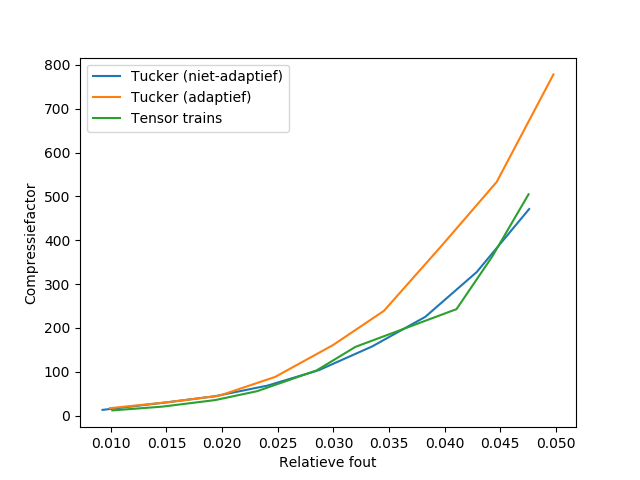
\includegraphics[scale=0.7]{images/tucker_vs_tensor_trains_Indian_Pines.png}
  \caption{Vergelijking tussen Tucker-gebaseerde compressie en tensor-train-compressie voor Indian Pines.}
\label{fig:tucker-vs-tensor-trains-indian-pines}
\end{figure}

\begin{figure}[]
  \centering
  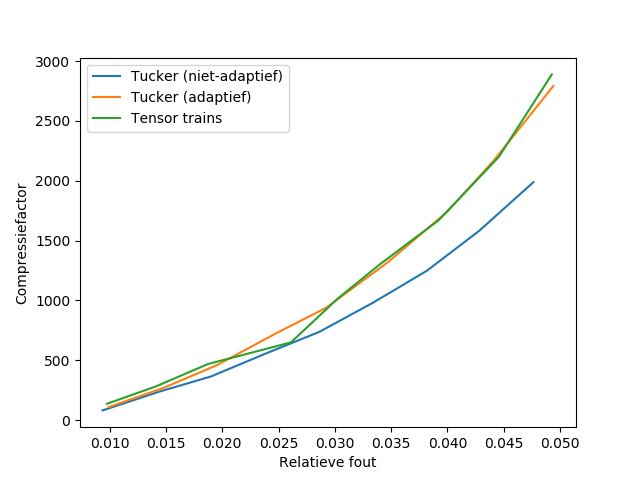
\includegraphics[scale=0.7]{images/tucker_vs_tensor_trains_Cuprite.png}
  \caption{Vergelijking tussen Tucker-gebaseerde compressie en tensor-train-compressie voor Cuprite.}
\label{fig:tucker-vs-tensor-trains-cuprite}
\end{figure}

\begin{figure}[]
  \centering
  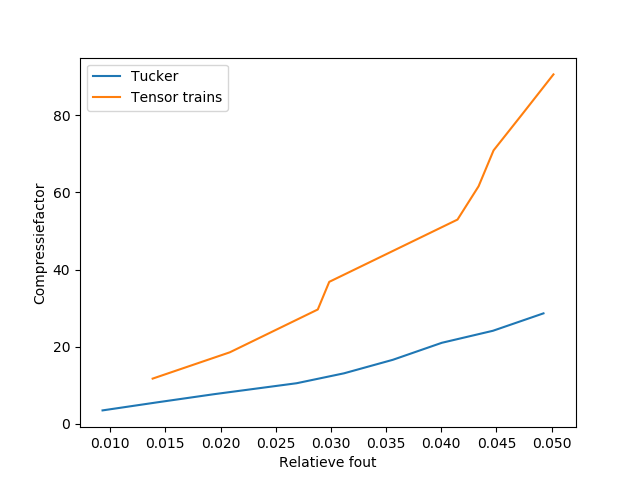
\includegraphics[scale=0.7]{images/tucker_vs_tensor_trains_Pavia_Centre.png}
  \caption{Vergelijking tussen Tucker-gebaseerde compressie en tensor-train-compressie voor Pavia Centre.}
\label{fig:tucker-vs-tensor-trains-pavia-centre}
\end{figure}

\begin{figure}[]
  \centering
  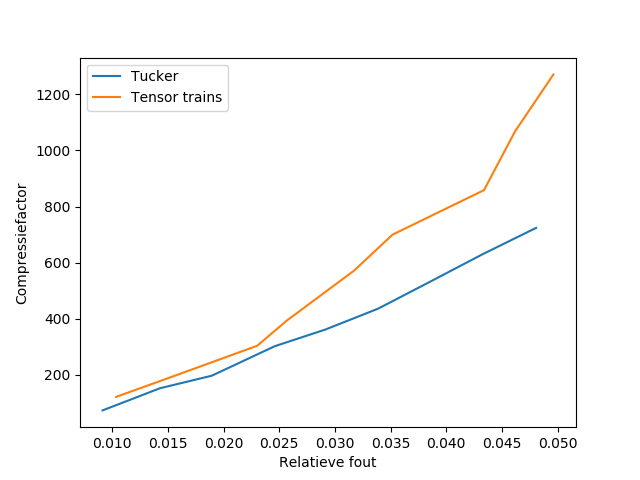
\includegraphics[scale=0.7]{images/tucker_vs_tensor_trains_Mauna_Kea.png}
  \caption{Vergelijking tussen Tucker-gebaseerde compressie en tensor-train-compressie voor Mauna Kea.}
\label{fig:tucker-vs-tensor-trains-mauna-kea}
\end{figure}

\begin{figure}[]
\centering
\begin{subfigure}{0.48\textwidth}
  \centering
  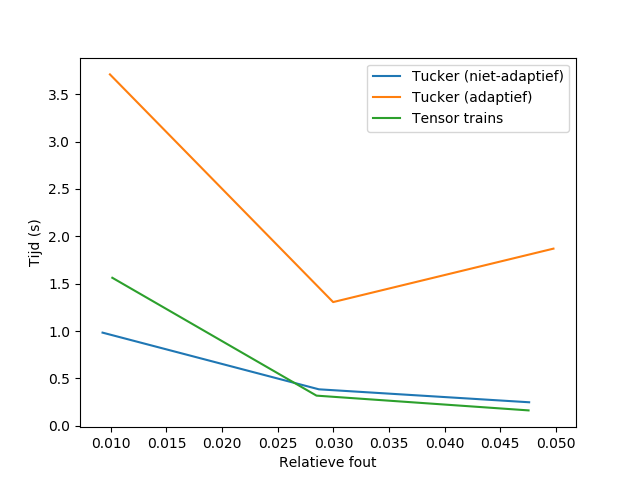
\includegraphics[width=\linewidth]{images/tucker_vs_tensor_trains_times_Indian_Pines.png}
  \caption{Indian Pines}
\end{subfigure}
\begin{subfigure}{0.48\textwidth}
  \centering
  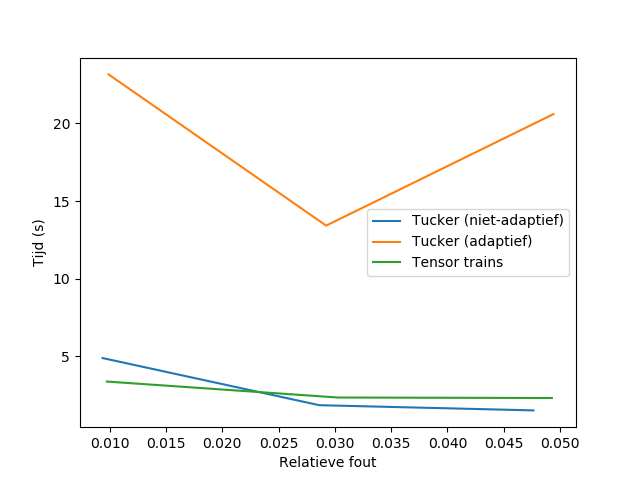
\includegraphics[width=\linewidth]{images/tucker_vs_tensor_trains_times_Cuprite.png}
  \caption{Cuprite}
\end{subfigure}
\\
\begin{subfigure}{0.48\textwidth}
  \centering
  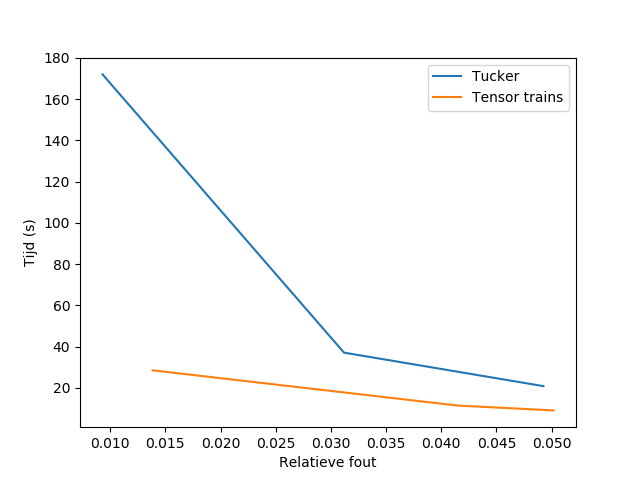
\includegraphics[width=\linewidth]{images/tucker_vs_tensor_trains_times_Pavia_Centre.png}
  \caption{Pavia Centre}
\end{subfigure}
\begin{subfigure}{0.48\textwidth}
  \centering
  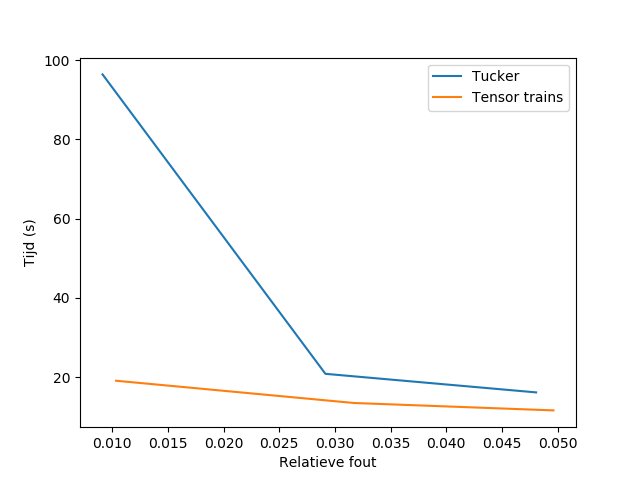
\includegraphics[width=\linewidth]{images/tucker_vs_tensor_trains_times_Mauna_Kea.png}
  \caption{Mauna Kea}
\end{subfigure}
\caption{Compressietijd in functie van relatieve fout voor Tucker-compressie en tensor trains (uitgemiddeld over 3 experimenten).}
\label{fig:tucker-vs-tensor-trains-times}
\end{figure}

\section{Vergelijking met algemene lossy compressie}

In deze sectie zullen we kort enkele algemene lossy-compressie-methoden bespreken, gevolgd door een vergelijking met onze tensor-train-gebaseerde compressie.

\newpage
\subsection{JPEG}

We hebben JPEG \cite{ref:jpeg} al aangehaald in hoofdstuk \ref{hoofdstuk:achtergrond}, maar nu leggen we uit hoe men hiermee een simpel algoritme kan maken voor het comprimeren van hyperspectrale afbeeldingen. Eerst verschuiven en schalen we de originele data, gevolgd door afronding, zodat elke waarde zich bevindt in het domein $\{0, 1, \dots, 255\}$. Deze quantisatie cre\"eert een fout die verwaarloosbaar is voor onze toepassingen. Daarna splitsen we de spectrale banden op in groepen van drie, comprimeren elke groep als \'e\'en RGB-afbeelding met JPEG en slaan de reeks gecomprimeerde afbeeldingen op. Bij de compressie wordt een kwaliteitsparameter opgegeven tussen 1 (slechtste kwaliteit) en 95 (beste kwaliteit). Deze methode houdt alleen rekening met de correlatie tussen de spectrale banden binnen elke groep, waardoor erg veel redundantie niet benut wordt en men geen goede compressie moet verwachten.

\newpage
\subsection{Videocompressie met x264}

Een betere manier om met algemene compressie de correlatie tussen de spectrale banden te gebruiken, is aan de hand van videocompressie. Een typische video bestaat namelijk uit een reeks \textit{frames} waarbij opeenvolgende frames erg op elkaar lijken, terwijl hyperspectrale afbeeldingen bestaan uit een reeks spectrale banden die allemaal qua structuur op elkaar lijken. Bovendien heeft videocompressie erg belangrijke toepassingen en wordt er al decennia met veel aandacht onderzoek gedaan in dit domein, dus men kan zich voorstellen dat moderne \textit{video codecs} erg effici\"ent zijn.\\

Concreet zullen we (zoals bij de JPEG-methode) eerst de volledige tensor quantiseren naar 8 bits, waarna we elke spectrale band doorgeven als een frame aan ffmpeg \cite{ref:ffmpeg}, een uitgebreid en veel-gebruikt programma voor het verwerken van audio en video. Voor de compressie gebruiken we de video codec x264 \cite{ref:x264}. Deze compressie gebeurt op basis van de CRF-parameter (\textit{constant rate factor}), die de afweging tussen de compressiefout en de grootte van de uitvoer bepaalt. Een CRF-waarde van 0 komt neer op lossless compressie, een waarde van 51 (het maximum) geeft de slechtste kwaliteit. Daarnaast heeft ffmpeg ook een preset-parameter, die bepaalt hoe belangrijk de compressietijd is ten opzichte van de compressiefactor en -fout. We zullen hiervoor zowel de standaardoptie \textit{medium} als de snelste optie \textit{ultrafast} proberen.

\subsection{Vergelijking}

In figuren \ref{fig:general-comparison-indian-pines}, \ref{fig:general-comparison-cuprite}, \ref{fig:general-comparison-pavia-centre} en \ref{fig:general-comparison-mauna-kea} zien we de algemene vergelijkingen op vlak van compressiefout en -factor. Zoals verwacht doet de JPEG-methode het erg slecht, dus hier zullen we verder geen rekening mee houden. Videocompressie aan de hand van x264 met preset medium scoort echter wel hoog en geeft ongeveer even goede compressie als tensor trains. Aan de andere kant zien we dat de preset ultrafast veel slechtere resultaten geeft. De resultaten van Tucker-gebaseerde compressie zijn weer even goed tot slechter dan bij tensor trains, zoals besproken in de vorige sectie, waar we ook al leerden dat deze methode trager was. Het is dus de vraag wat de verschillen in compressietijd tussen tensor trains en videocompressie dan zijn.\\

Het antwoord hierop vindt men in figuur \ref{fig:general-comparison-times}. Als het gaat om videocompressie zijn de resultaten consistent: de preset ultrafast is elke keer significant sneller dan medium. Daarnaast heeft de CRF-parameter ook slechts een beperkte invloed op de compressietijd. Dit ligt anders bij tensor trains: we merken dat de compressietijd hierbij sterker daalt in functie van de relatieve fout. Daarnaast zijn tensor trains sneller dan videocompressie voor goed comprimeerbare datasets (zie Cuprite en Mauna Kea) maar trager voor slecht comprimeerbare (zie Pavia Centre). Als men deze twee zaken combineert, kan men concluderen dat de compressietijd van onze methode met tensor trains sterk afhankelijk is van de grootte van de uitvoer van de ST-HOSVD en dat een significante hoeveelheid tijd besteed wordt aan het quantiseren en encoderen van deze uitvoer.

\newpage
\begin{figure}[H]
  \centering
  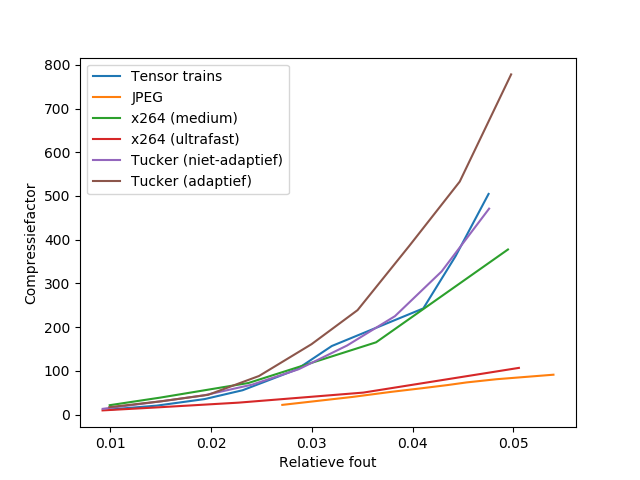
\includegraphics[scale=0.7]{images/general_comparison_new_Indian_Pines.png}
  \caption{Vergelijking tussen tensor trains en algemene compressiemethoden voor Indian Pines.}
\label{fig:general-comparison-indian-pines}
\end{figure}

\begin{figure}[H]
  \centering
  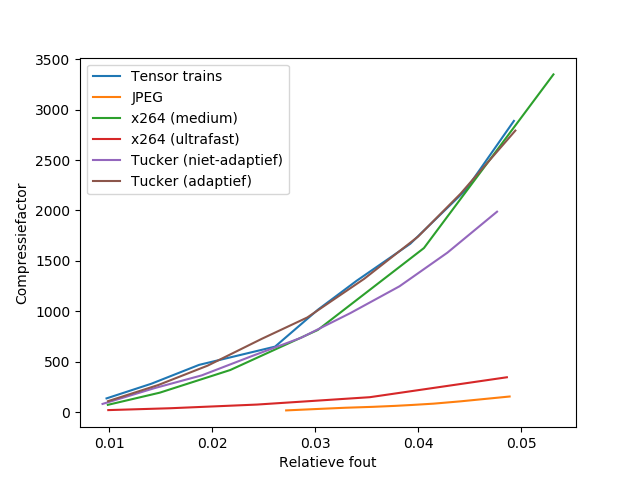
\includegraphics[scale=0.7]{images/general_comparison_new_Cuprite.png}
  \caption{Vergelijking tussen tensor trains en algemene compressiemethoden voor Cuprite.}
\label{fig:general-comparison-cuprite}
\end{figure}

\begin{figure}[H]
  \centering
  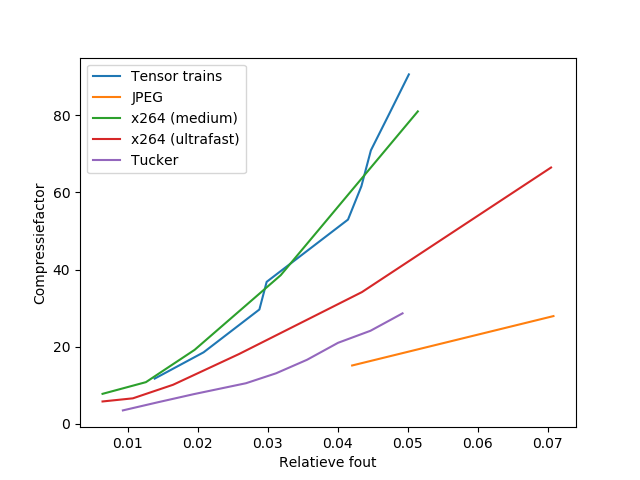
\includegraphics[scale=0.7]{images/general_comparison_new_Pavia_Centre.png}
  \caption{Vergelijking tussen tensor trains en algemene compressiemethoden voor Pavia Centre.}
\label{fig:general-comparison-pavia-centre}
\end{figure}

\begin{figure}[H]
  \centering
  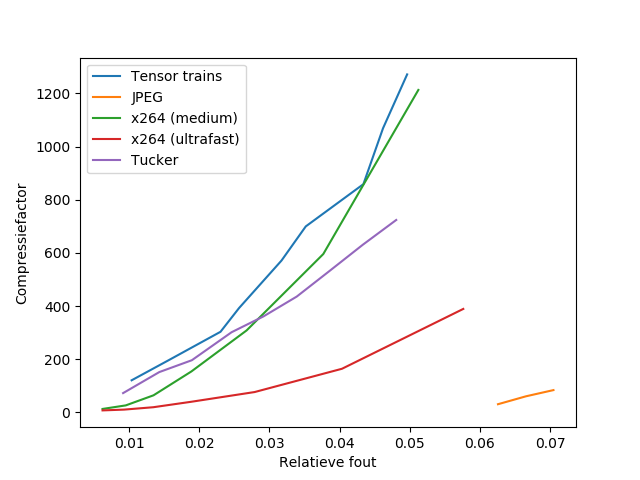
\includegraphics[scale=0.7]{images/general_comparison_new_Mauna_Kea.png}
  \caption{Vergelijking tussen tensor trains en algemene compressiemethoden voor Mauna Kea.}
\label{fig:general-comparison-mauna-kea}
\end{figure}

\begin{figure}[H]
\centering
\begin{subfigure}{0.48\textwidth}
  \centering
  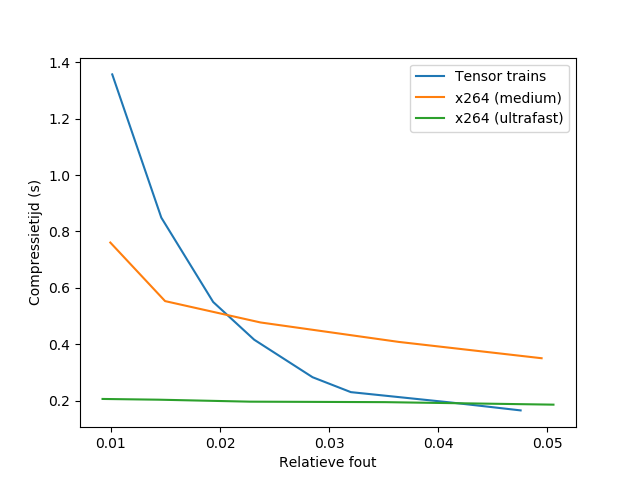
\includegraphics[width=\linewidth]{images/general_comparison_times_Indian_Pines.png}
  \caption{Indian Pines}
\end{subfigure}
\begin{subfigure}{0.48\textwidth}
  \centering
  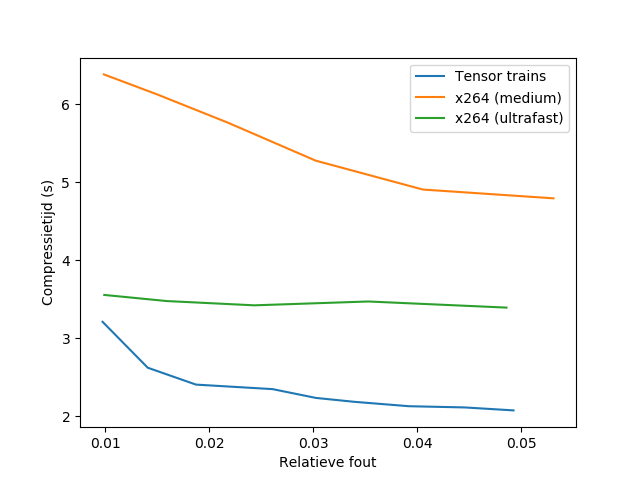
\includegraphics[width=\linewidth]{images/general_comparison_times_Cuprite.png}
  \caption{Cuprite}
\end{subfigure}
\\
\begin{subfigure}{0.48\textwidth}
  \centering
  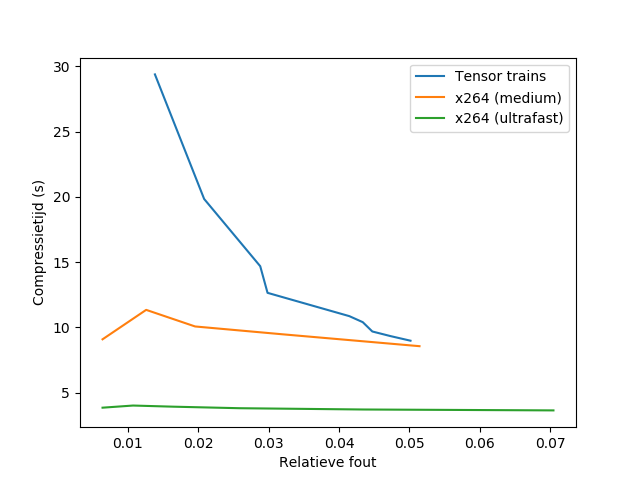
\includegraphics[width=\linewidth]{images/general_comparison_times_Pavia_Centre.png}
  \caption{Pavia Centre}
\end{subfigure}
\begin{subfigure}{0.48\textwidth}
  \centering
  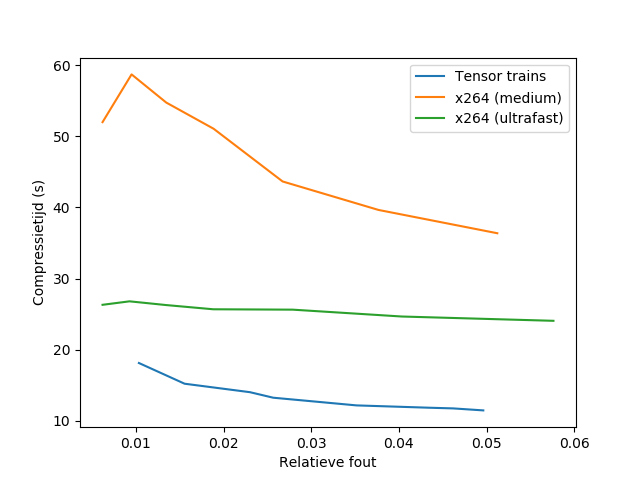
\includegraphics[width=\linewidth]{images/general_comparison_times_Mauna_Kea.png}
  \caption{Mauna Kea}
\end{subfigure}
\caption{Compressietijd in functie van relatieve fout voor tensor trains en videocompressie (uitgemiddeld over 10 experimenten).}
\label{fig:general-comparison-times}
\end{figure}

Ten slotte besloten we om ook eens te kijken naar de decompressietijd in figuur \ref{fig:general-comparison-decompression-times}. Opnieuw is de uitvoeringstijd van tensor trains erg afhankelijk van de relatieve fout, terwijl dit bij videocompressie minder invloed heeft. Verder heeft, zoals verwacht, de preset van ffmpeg erg weinig effect op de decompressietijd; deze parameter is namelijk alleen bedoeld om de compressietijd te controleren. We concluderen dat videocompressie over het algemeen veel sneller kan decomprimeren, maar dit verschil wordt kleiner bij grote datasets (zie Mauna Kea).

\newpage
\begin{figure}[H]
\centering
\begin{subfigure}{0.48\textwidth}
  \centering
  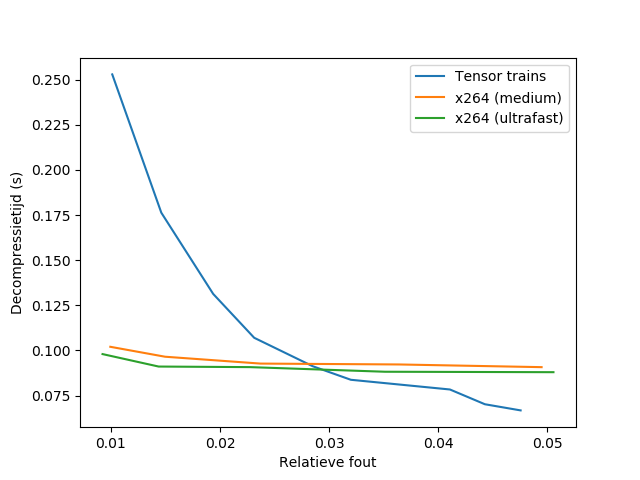
\includegraphics[width=\linewidth]{images/general_comparison_decompression_times_Indian_Pines.png}
  \caption{Indian Pines}
\end{subfigure}
\begin{subfigure}{0.48\textwidth}
  \centering
  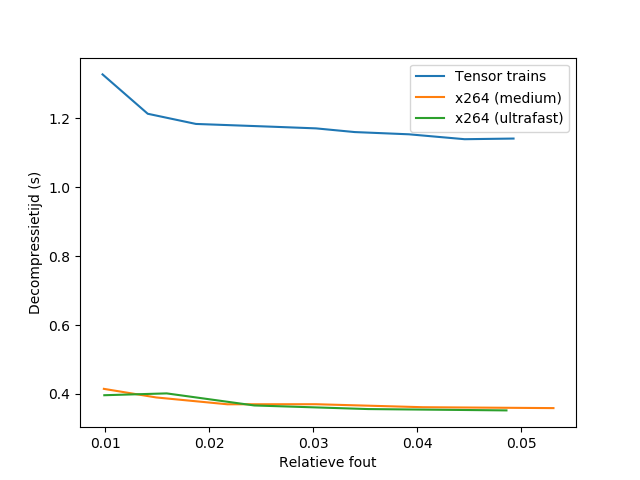
\includegraphics[width=\linewidth]{images/general_comparison_decompression_times_Cuprite.png}
  \caption{Cuprite}
\end{subfigure}
\\
\begin{subfigure}{0.48\textwidth}
  \centering
  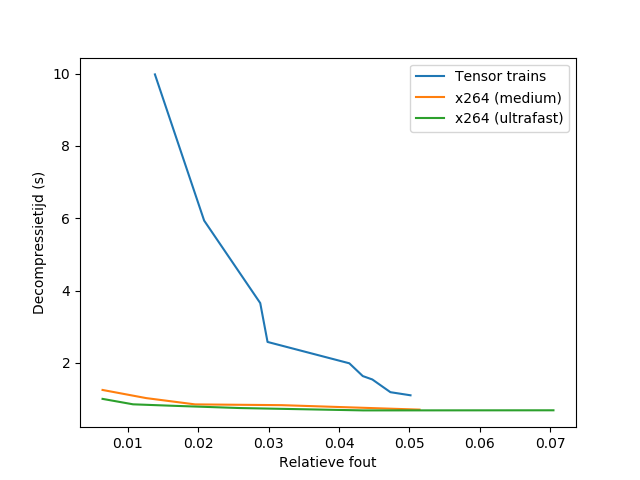
\includegraphics[width=\linewidth]{images/general_comparison_decompression_times_Pavia_Centre.png}
  \caption{Pavia Centre}
\end{subfigure}
\begin{subfigure}{0.48\textwidth}
  \centering
  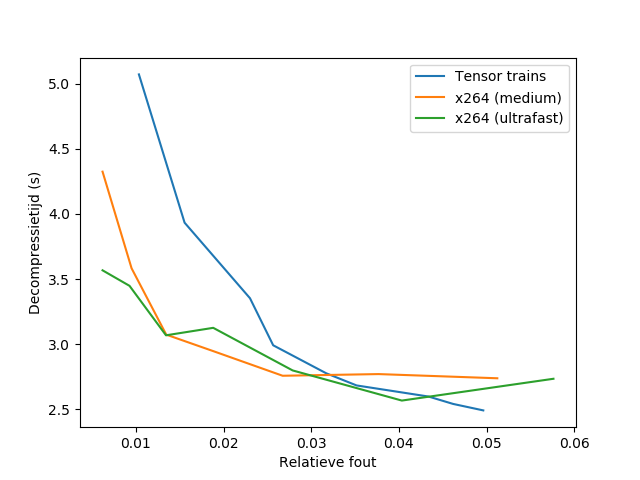
\includegraphics[width=\linewidth]{images/general_comparison_decompression_times_Mauna_Kea.png}
  \caption{Mauna Kea}
\end{subfigure}
\caption{Decompressietijd in functie van relatieve fout voor tensor trains en videocompressie (uitgemiddeld over 10 experimenten).}
\label{fig:general-comparison-decompression-times}
\end{figure}

\section{Voorbeeldcompressies}

Om dit hoofdstuk af te sluiten zullen we nog een aantal hyperspectrale afbeeldingen tonen voor en na compressie met tensor trains. Zoals in hoofdstuk \ref{hoofdstuk:methodologie} zullen we deze voorstellen door de spectrale banden op te tellen en deze sommen te verschuiven en schalen naar het domein $\{0, \dots, 255\}$. In deze sectie zullen relatieve fout en compressiefactor afgekort worden tot RF en CF respectievelijk.

\newpage
\begin{figure}[]
\centering
\begin{subfigure}{0.48\textwidth}
  \centering
  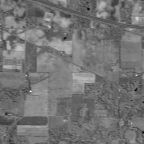
\includegraphics[scale=1]{images/indian_pines_cropped_sum.png}
  \caption{Origineel, 8910KB}
\end{subfigure}
\begin{subfigure}{0.48\textwidth}
  \centering
  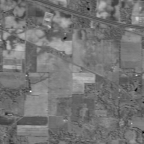
\includegraphics[scale=1]{images/example_compression_Indian_Pines_0_01.png}
  \caption{RF: 0.0101, CF: 12.15, 733.3KB}
\end{subfigure}
\\
\begin{subfigure}{0.48\textwidth}
  \centering
  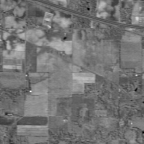
\includegraphics[scale=1]{images/example_compression_Indian_Pines_0_025.png}
  \caption{RF: 0.0231, CF: 55.89, 159.4KB}
\end{subfigure}
\begin{subfigure}{0.48\textwidth}
  \centering
  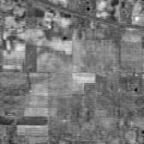
\includegraphics[scale=1]{images/example_compression_Indian_Pines_0_05.png}
  \caption{RF: 0.0475, CF: 504.75, 17.7KB}
\end{subfigure}
\caption{Voorbeeldcompressies van Indian Pines \cite{ref:ehu_aviris}.}
\end{figure}

\begin{figure}[]
\centering
\begin{subfigure}{\textwidth}
  \centering
  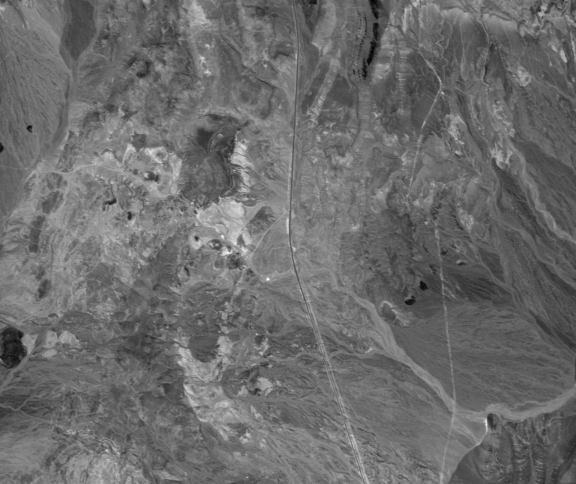
\includegraphics[scale=0.55]{images/cuprite_cropped_sum.png}
  \caption{Origineel, 103455KB}
\end{subfigure}
\\
\begin{subfigure}{\textwidth}
  \centering
  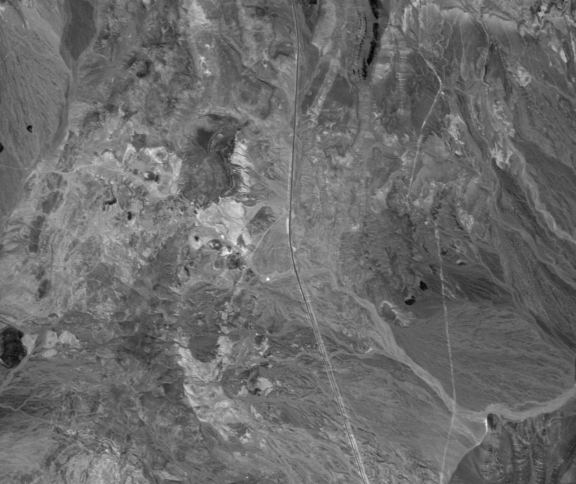
\includegraphics[scale=0.55]{images/example_compression_Cuprite_0_01.png}
  \caption{RF: 0.0098, CF: 136.2, 759.3KB}
\end{subfigure}
\end{figure}
\begin{figure}[]
\centering
\ContinuedFloat
\begin{subfigure}{\textwidth}
  \centering
  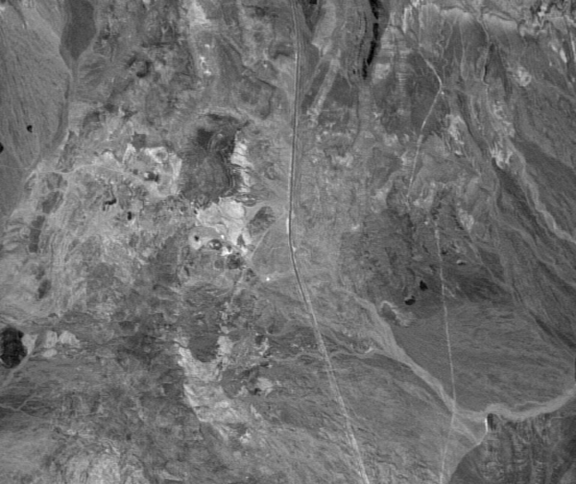
\includegraphics[scale=0.55]{images/example_compression_Cuprite_0_025.png}
  \caption{RF: 0.0261, CF: 649.6, 159.3KB}
\end{subfigure}
\begin{subfigure}{\textwidth}
  \centering
  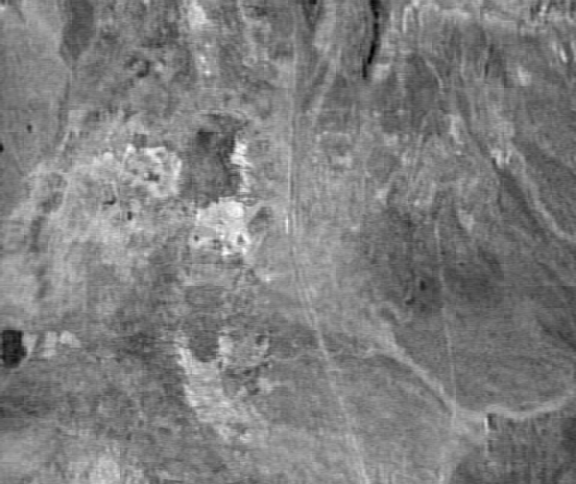
\includegraphics[scale=0.55]{images/example_compression_Cuprite_0_05.png}
  \caption{RF: 0.0493, CF: 2888.5, 35.8KB}
\end{subfigure}
\caption{Voorbeeldcompressies van Cuprite \cite{ref:ehu_aviris}.}
\end{figure}

\begin{figure}[]
\centering
\begin{subfigure}{\textwidth}
  \centering
  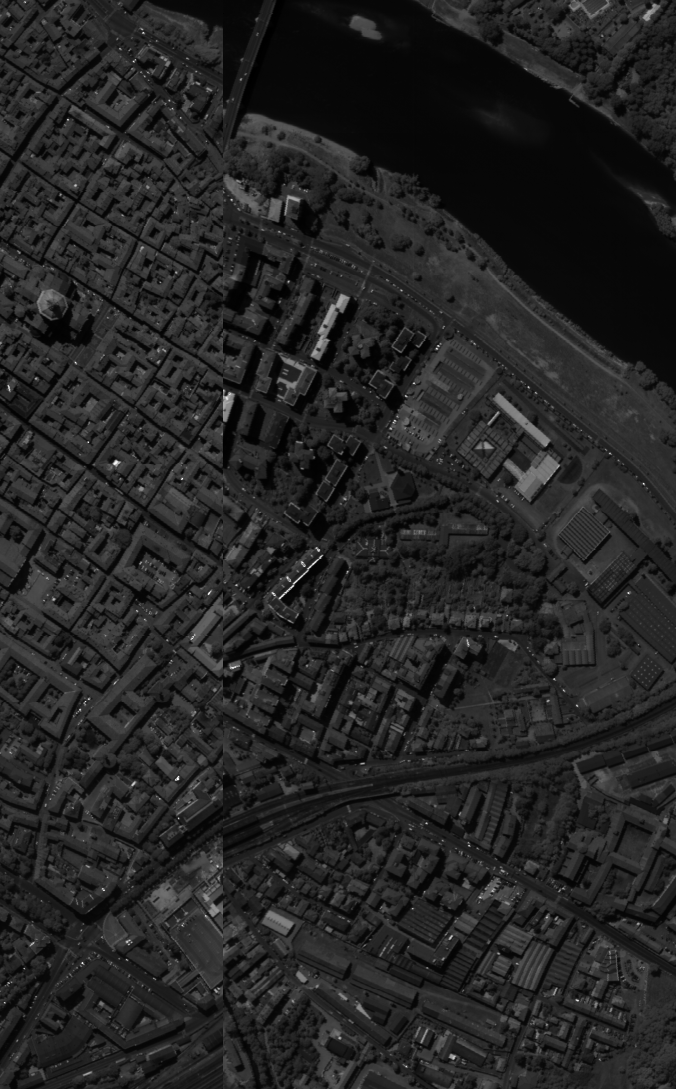
\includegraphics[width=0.85\linewidth]{images/pavia_sum.png}
  \caption{Origineel, 146657.7KB}
\end{subfigure}
\end{figure}
\begin{figure}[]
\centering
\ContinuedFloat
\begin{subfigure}{\textwidth}
  \centering
  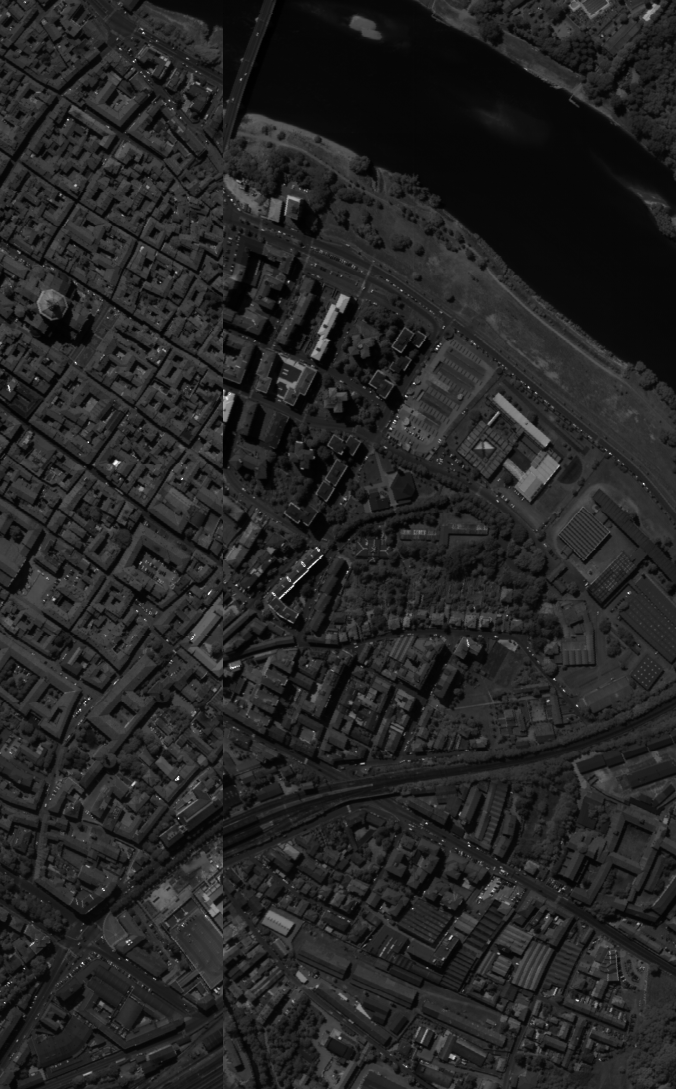
\includegraphics[width=0.85\linewidth]{images/example_compression_Pavia_Centre_0_01.png}
  \caption{RF: 0.0138, CF: 11.67, 12569.8KB}
\end{subfigure}
\end{figure}
\begin{figure}[]
\centering
\ContinuedFloat
\begin{subfigure}{\textwidth}
  \centering
  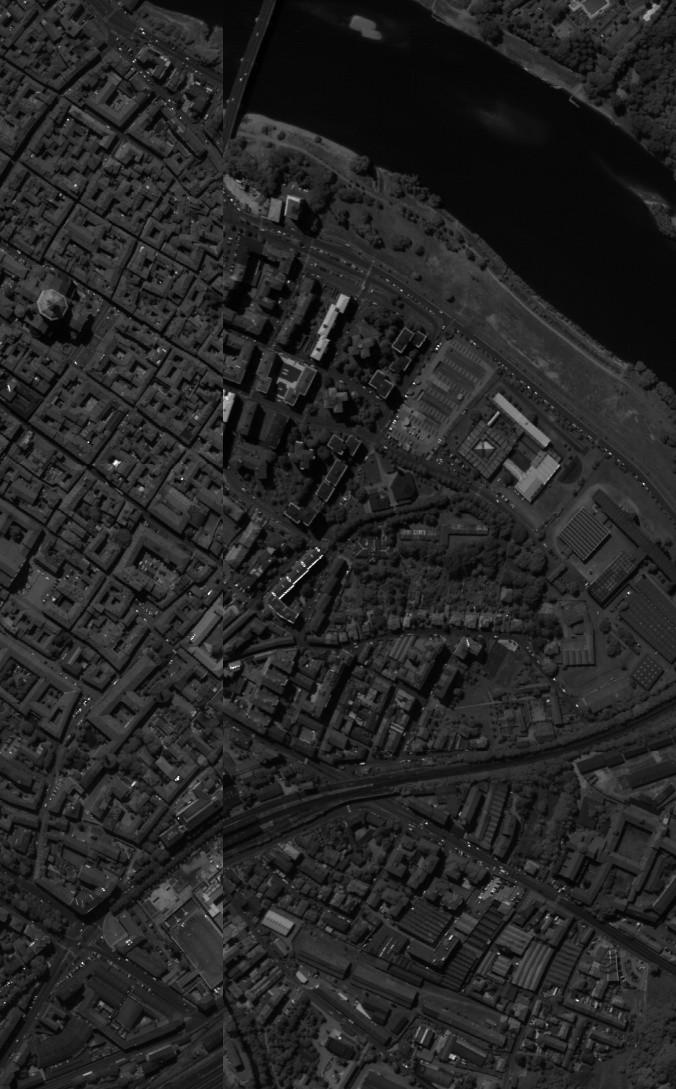
\includegraphics[width=0.85\linewidth]{images/example_compression_Pavia_Centre_0_025.png}
  \caption{RF: 0.0298, CF: 36.8, 3985.7KB}
\end{subfigure}
\end{figure}
\begin{figure}[]
\centering
\ContinuedFloat
\begin{subfigure}{\textwidth}
  \centering
  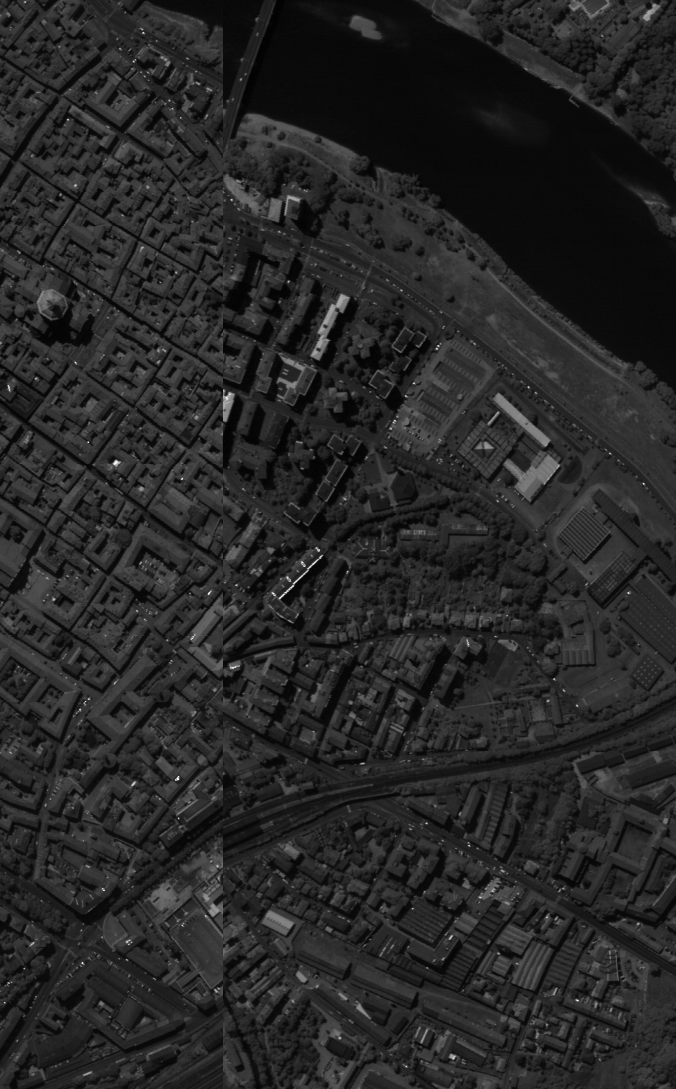
\includegraphics[width=0.85\linewidth]{images/example_compression_Pavia_Centre_0_05.png}
  \caption{RF: 0.0502, CF: 90.7, 1617.6KB}
\end{subfigure}
\caption{Voorbeeldcompressies van Pavia Centre \cite{ref:ehu_rosis}.}
\end{figure}

\begin{figure}[]
\centering
\begin{subfigure}{0.48\textwidth}
  \centering
  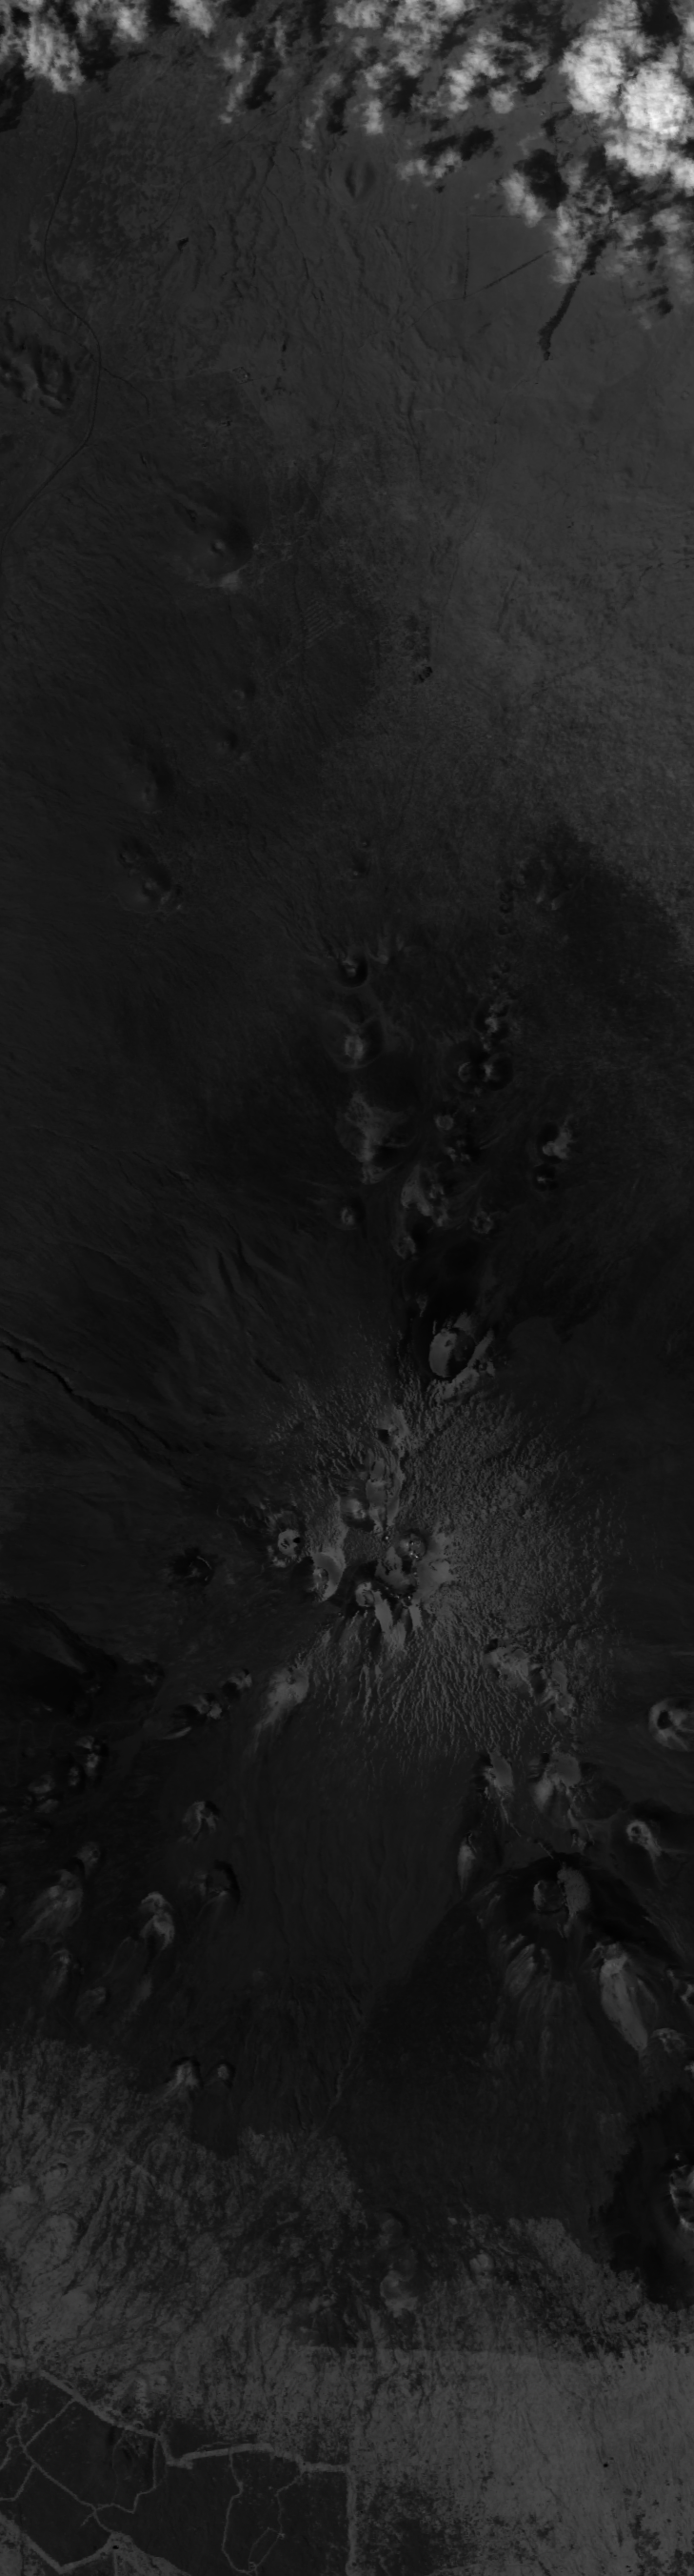
\includegraphics[width=0.8\linewidth]{images/mauna_kea_sum.png}
  \caption{Origineel, 766156.2KB}
\end{subfigure}
\begin{subfigure}{0.48\textwidth}
  \centering
  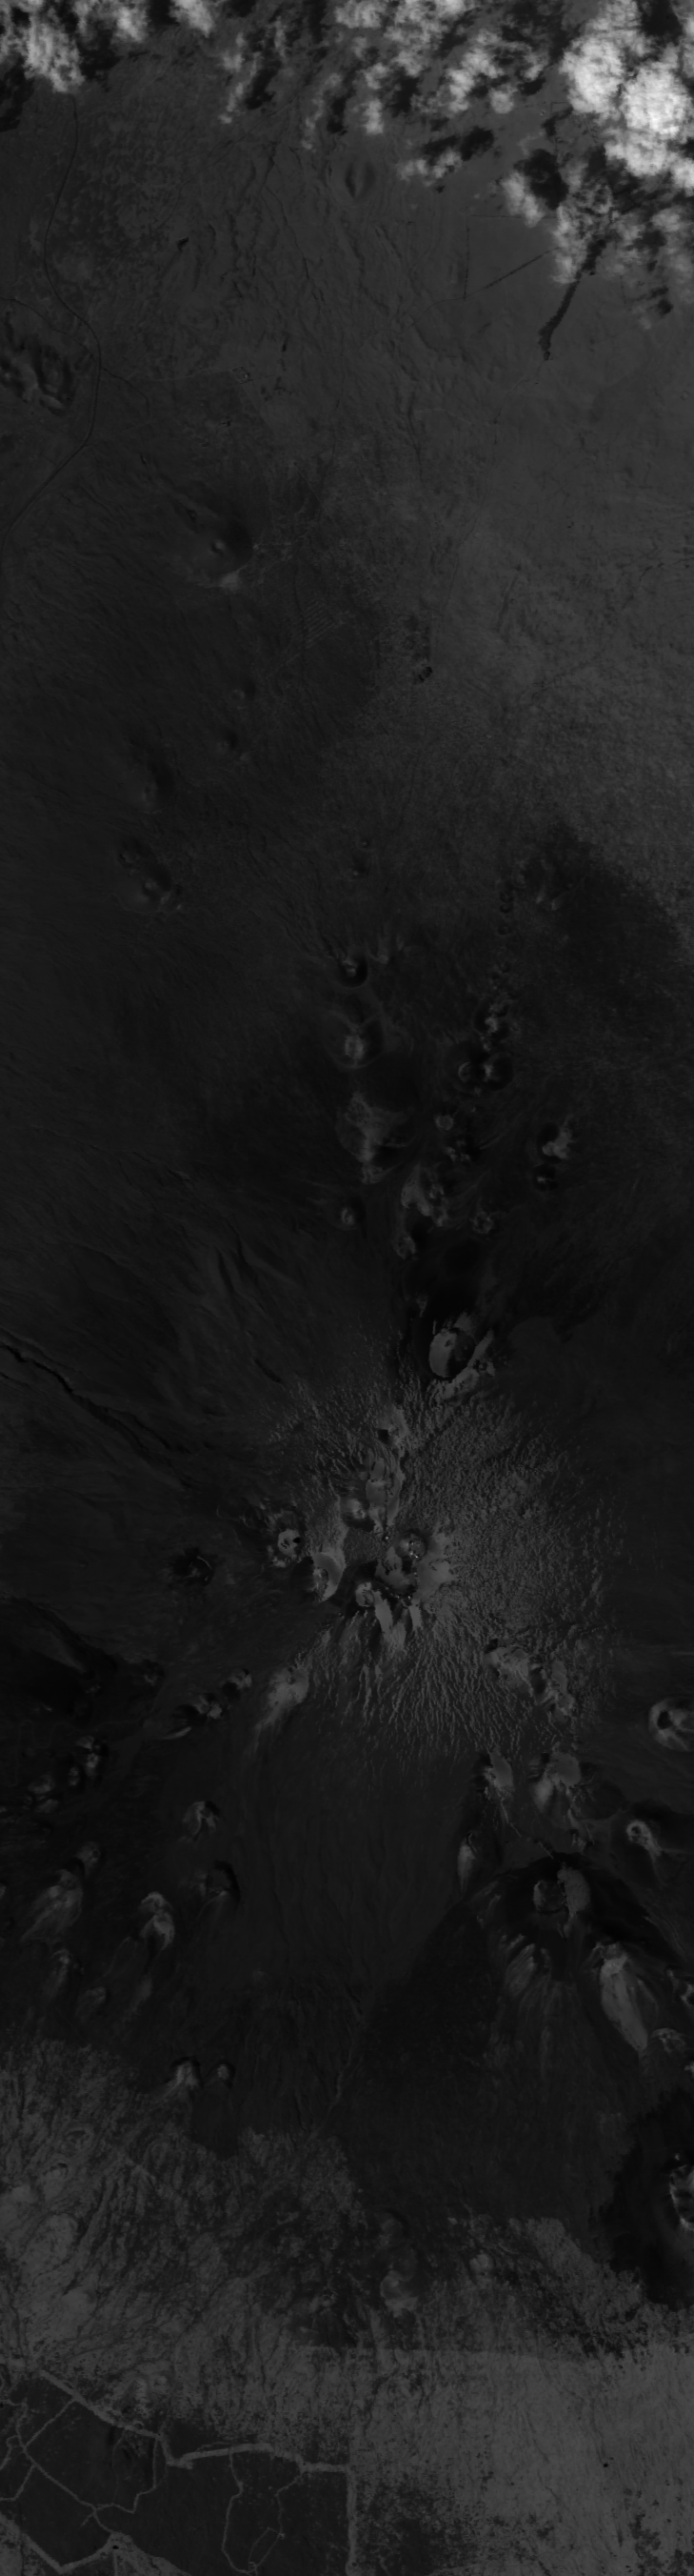
\includegraphics[width=0.8\linewidth]{images/example_compression_Mauna_Kea_0_01.png}
  \caption{RF: 0.0104, CF: 121, 6332.1KB}
\end{subfigure}
\end{figure}
\begin{figure}[]
\centering
\ContinuedFloat
\begin{subfigure}{0.48\textwidth}
  \centering
  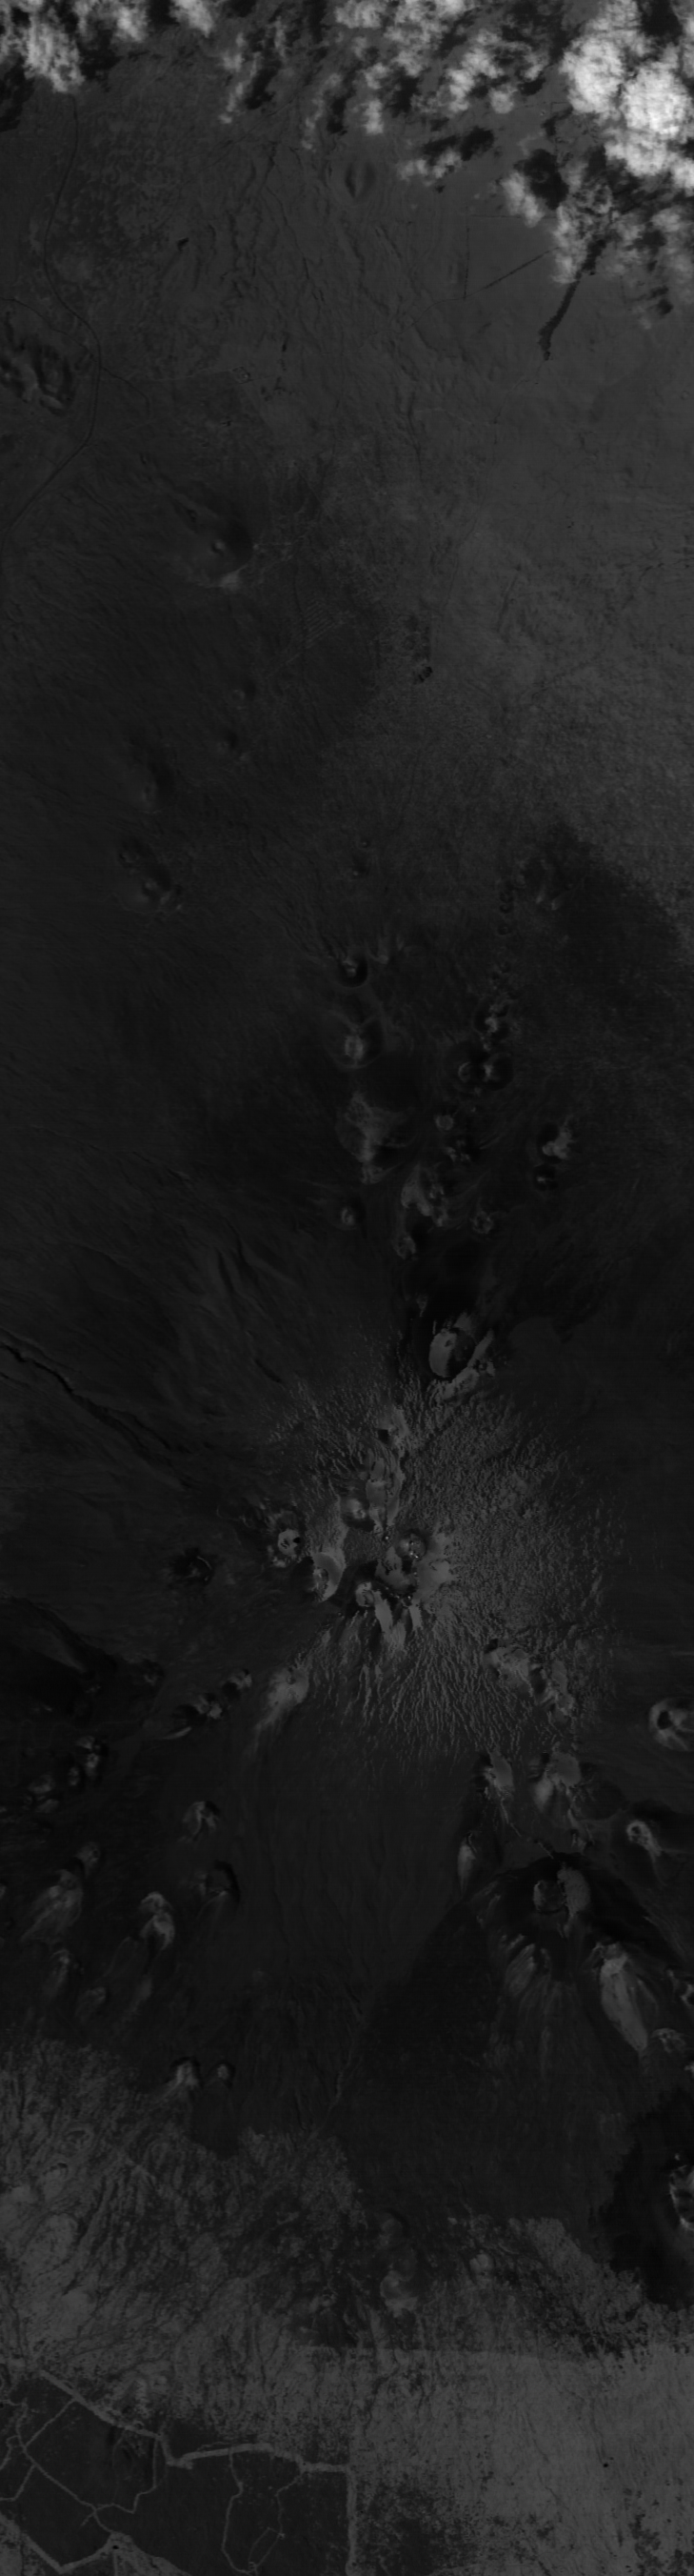
\includegraphics[width=0.8\linewidth]{images/example_compression_Mauna_Kea_0_025.png}
  \caption{RF: 0.0257, CF: 392.67, 1951.2KB}
\end{subfigure}
\begin{subfigure}{0.48\textwidth}
  \centering
  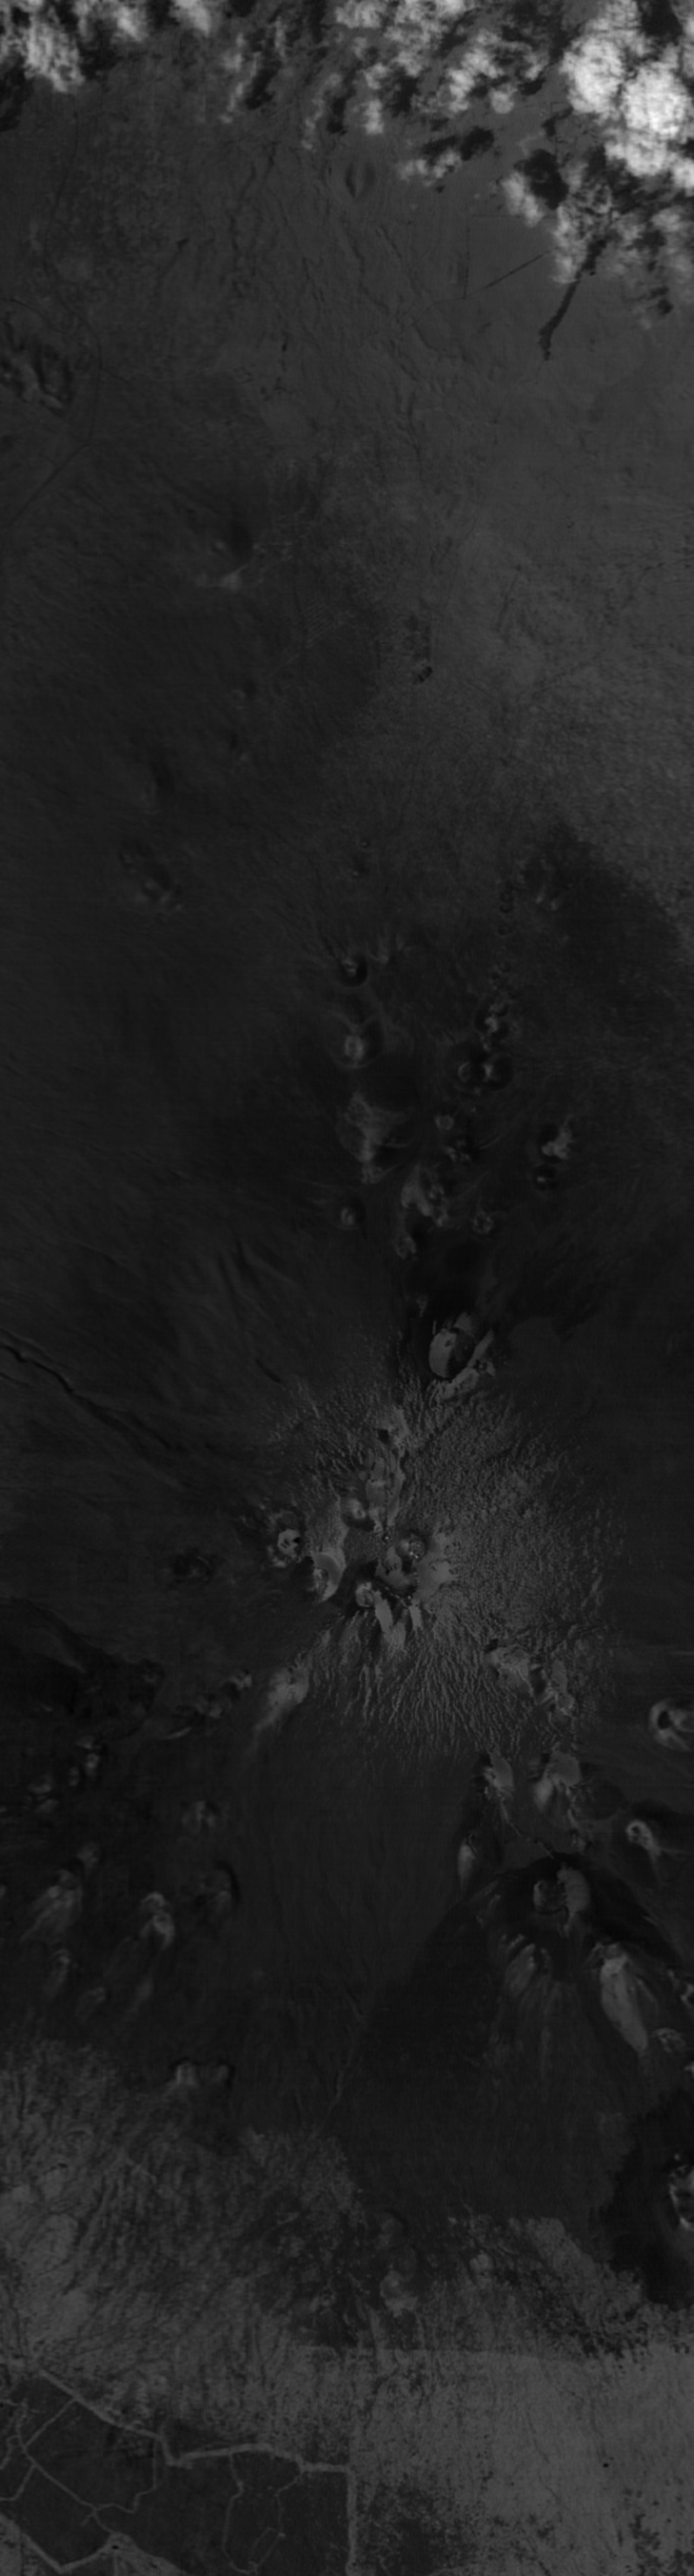
\includegraphics[width=0.8\linewidth]{images/example_compression_Mauna_Kea_0_05.png}
  \caption{RF: 0.0496, CF: 1271.31, 602.7KB}
\end{subfigure}
\caption{Voorbeeldcompressies van Mauna Kea \cite{ref:aviris}.}
\end{figure}